% Created 2022-05-02 Mon 11:12
% Intended LaTeX compiler: pdflatex
\documentclass[presentation,aspectratio=169]{beamer}
\usepackage[utf8]{inputenc}
\usepackage[T1]{fontenc}
\usepackage{graphicx}
\usepackage{grffile}
\usepackage{longtable}
\usepackage{wrapfig}
\usepackage{rotating}
\usepackage[normalem]{ulem}
\usepackage{amsmath}
\usepackage{textcomp}
\usepackage{amssymb}
\usepackage{capt-of}
\usepackage{hyperref}
\usepackage{khpreamble, euscript}
\DeclareMathOperator{\atantwo}{atan2}
\newcommand*{\ctrb}{\EuScript{C}}
\newcommand*{\obsv}{\EuScript{O}}
\usetheme{default}
\author{Kjartan Halvorsen}
\date{\today}
\title{Behavior trees}
\hypersetup{
 pdfauthor={Kjartan Halvorsen},
 pdftitle={Behavior trees},
 pdfkeywords={},
 pdfsubject={},
 pdfcreator={Emacs 26.3 (Org mode 9.4.6)}, 
 pdflang={English}}
\begin{document}

\maketitle

\section{Example behavior tree}
\label{sec:org72ffba7}

\begin{frame}[label={sec:orge11a71e}]{Ejemplo \emph{Pac-Man}}
\begin{center}
  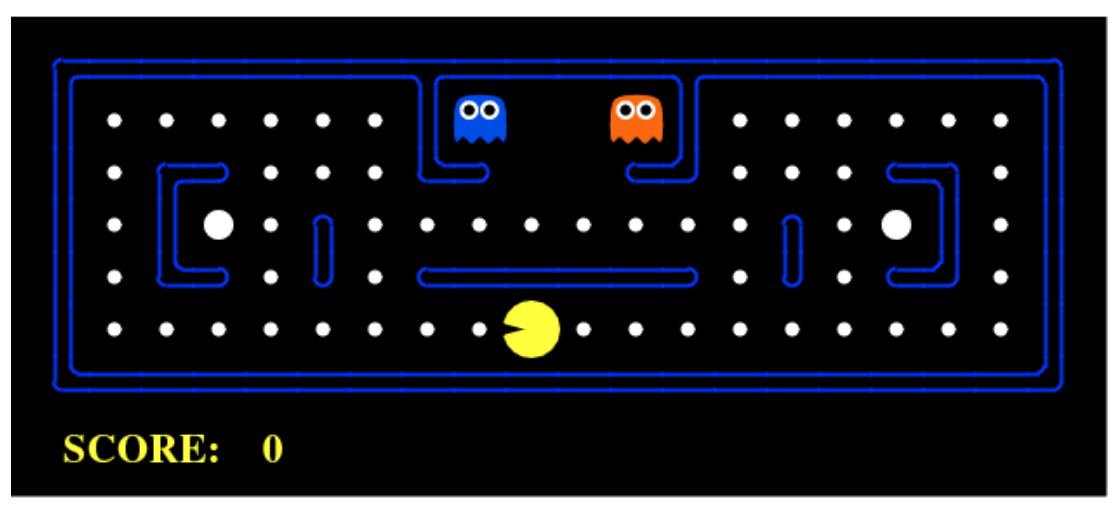
\includegraphics[width=.8\linewidth]{../figures/bt-book-fig-1_10.png}
\end{center}

{\footnotesize Capitulo 1.4 en Colledanchise y Ögren \emph{Behavior trees in robotics and AI}}
\end{frame}

\begin{frame}[label={sec:orgd91d00f}]{Ejemplo \emph{Pac-Man}}
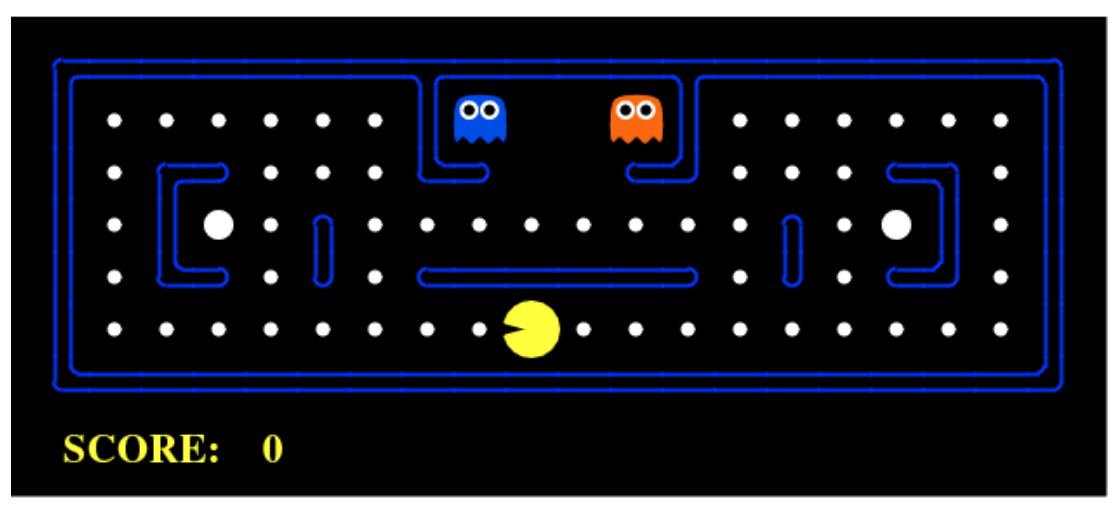
\includegraphics[width=0.4\linewidth]{../figures/bt-book-fig-1_10.png}

\begin{center}
  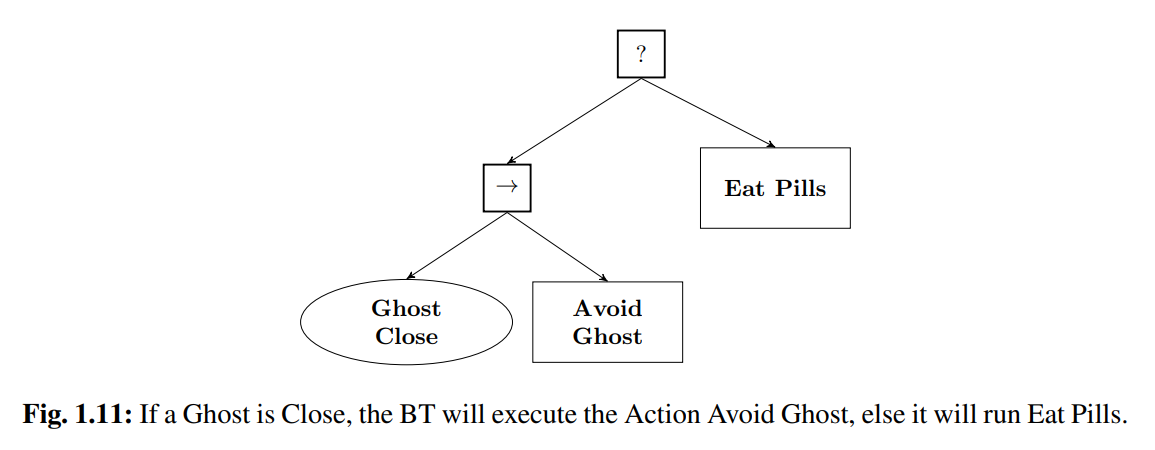
\includegraphics[width=.8\linewidth]{../figures/bt-book-fig-1_11.png}
\end{center}
\end{frame}

\begin{frame}[label={sec:org5ab115f}]{Ejemplo \emph{Pac-Man} modo combatitivo}
\begin{columns}
\begin{column}{0.6\columnwidth}
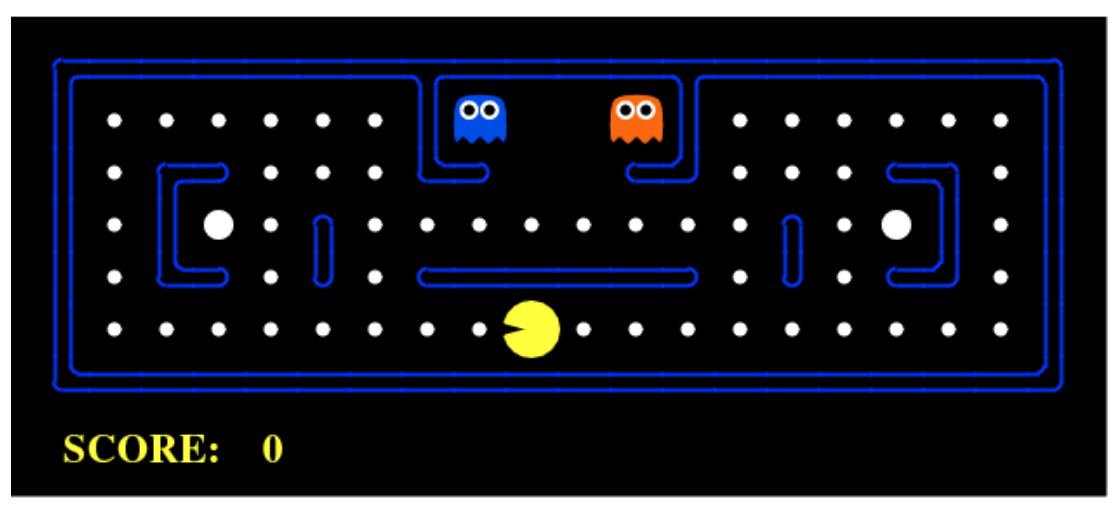
\includegraphics[width=0.6\linewidth]{../figures/bt-book-fig-1_10.png}

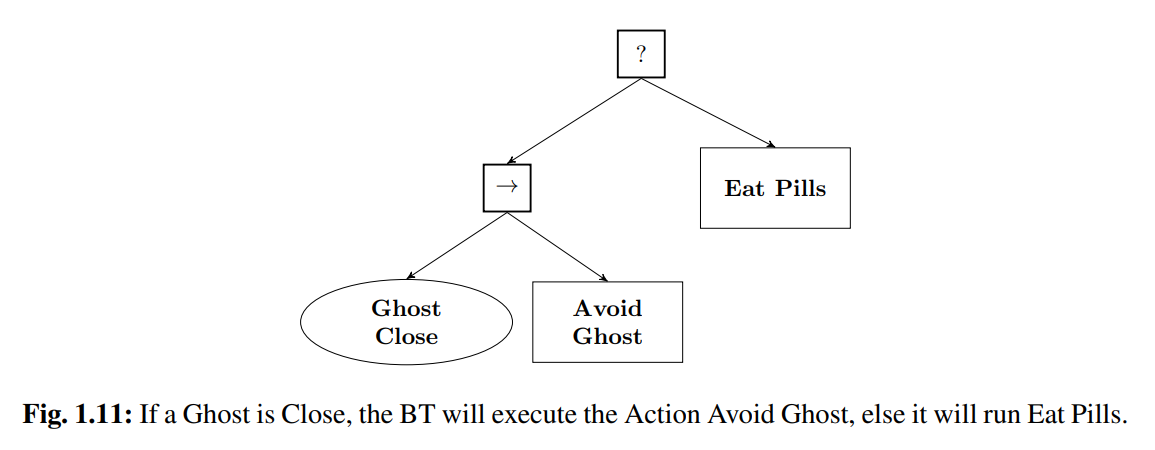
\includegraphics[width=\linewidth]{../figures/bt-book-fig-1_11.png}
\end{column}

\begin{column}{0.4\columnwidth}
\pause


\begin{center}
  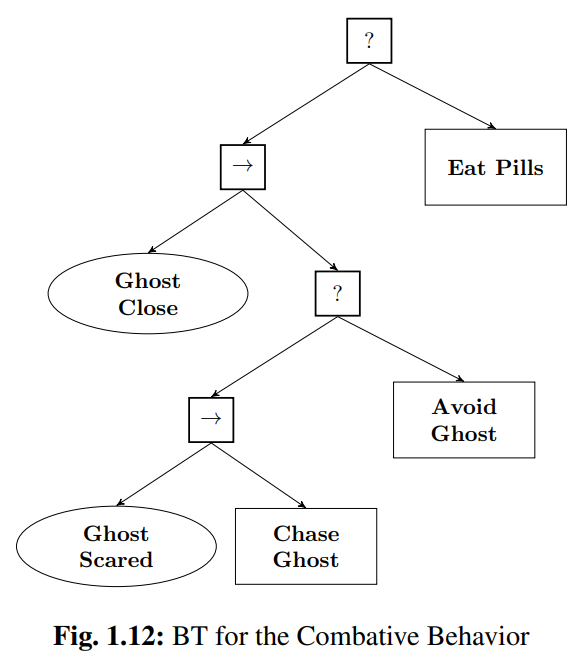
\includegraphics[width=\linewidth]{../figures/bt-book-fig-1_12.png}
\end{center}
\end{column}
\end{columns}
\end{frame}


\begin{frame}[label={sec:org81d3a07}]{Ejemplo \emph{Pick-and-place reto}}
\begin{center}
  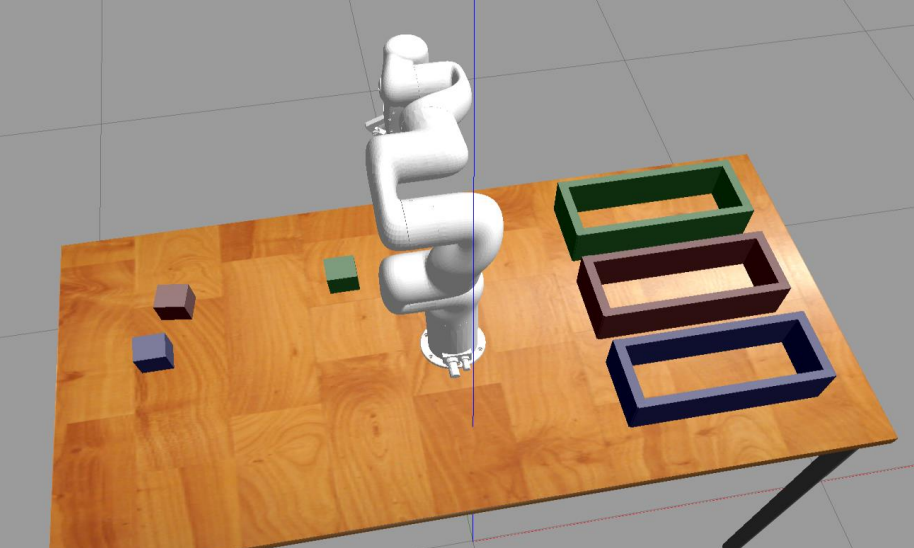
\includegraphics[width=0.8\linewidth]{../figures/reto-gazebo.png}
\end{center}
\end{frame}

\begin{frame}[label={sec:org873107f}]{Ejemplo \emph{Pick-and-place reto}}
\begin{center}
  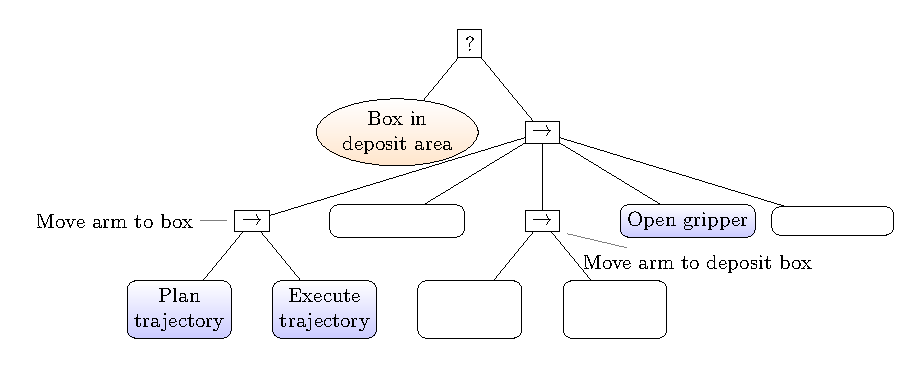
\includegraphics[width=\linewidth]{../figures/bt-manipulator-task-exercise}
\end{center}

\alert{Actividad} Llena las cajas vacías
\end{frame}


\begin{frame}[label={sec:orgf9f168d}]{Ejemplo \emph{Pick-and-place reto}}
\begin{center}
  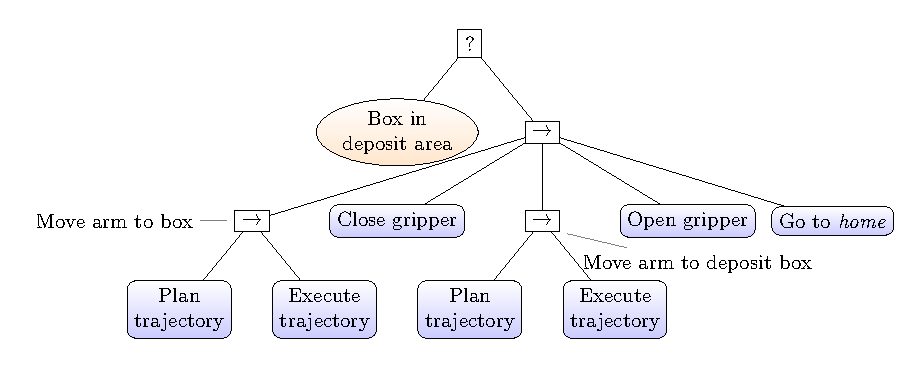
\includegraphics[width=\linewidth]{../figures/bt-manipulator-task}
\end{center}
\end{frame}

\begin{frame}[label={sec:org1de7139}]{Ejemplo \emph{Pick-and-place reto}}
Incluyendo más detalles

\begin{center}
  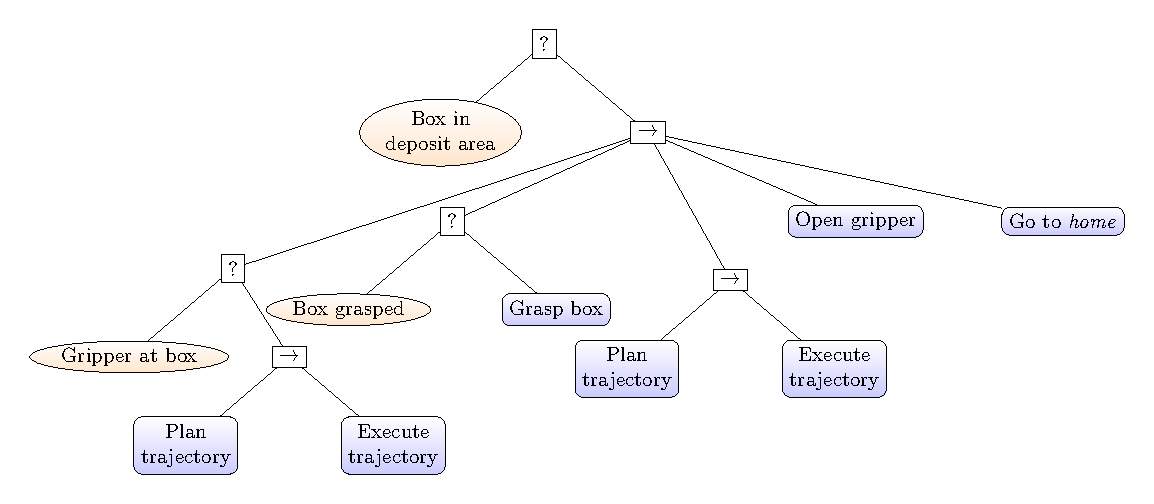
\includegraphics[width=\linewidth]{../figures/bt-manipulator-task-detailed}
\end{center}
\end{frame}


\begin{frame}[label={sec:org87043d6}]{Pure pursuit}
\begin{center}
  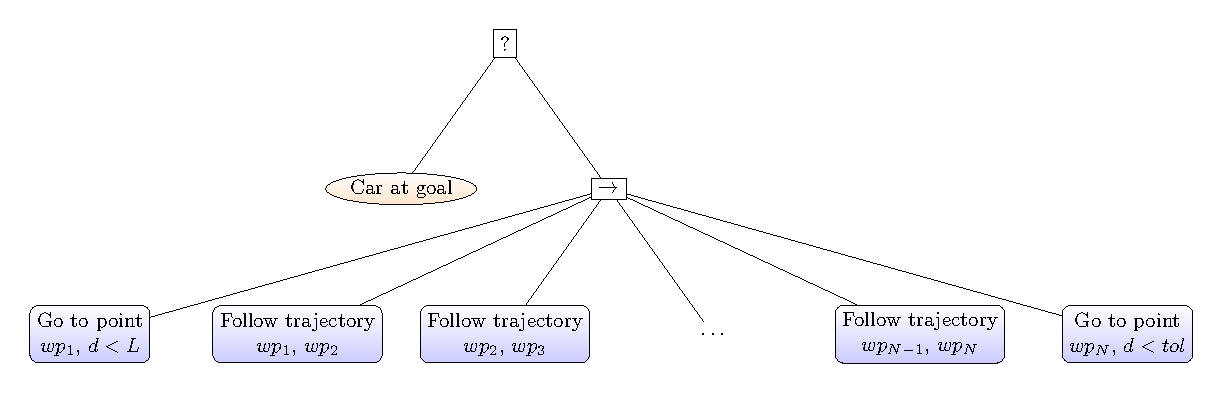
\includegraphics[width=\linewidth]{../figures/bt-pure-pursuit}
\end{center}
\end{frame}

\begin{frame}[label={sec:orgf252dcd}]{Pure pursuit}
Un problema posible

\begin{columns}
\begin{column}{0.4\columnwidth}
\begin{center}
  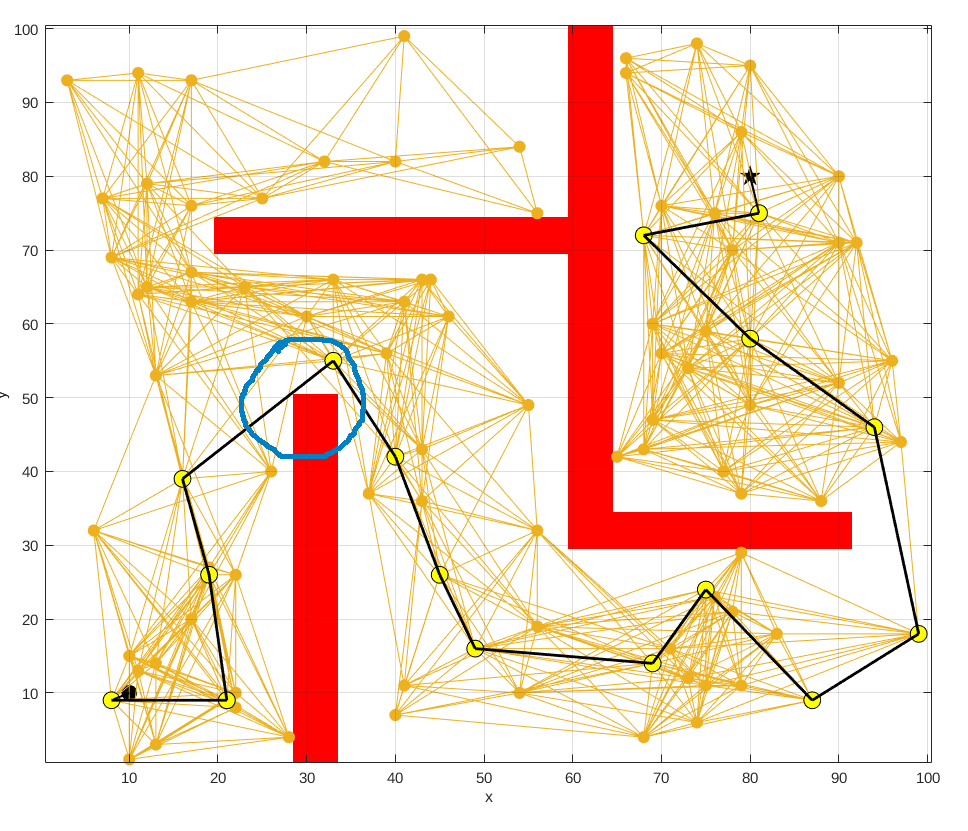
\includegraphics[width=\linewidth]{../figures/prm-example}
\end{center}
\end{column}

\begin{column}{0.6\columnwidth}
\pause
\begin{center}
  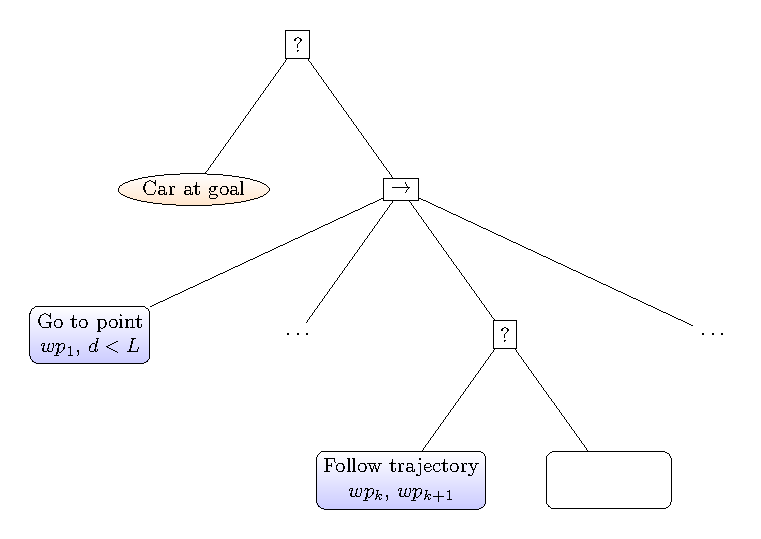
\includegraphics[width=\linewidth]{../figures/bt-pure-pursuit-collision-excercise}
\end{center}
\end{column}
\end{columns}
\end{frame}
\end{document}